\documentclass[border=10pt]{standalone}
\usepackage{tikz}
\begin{document}
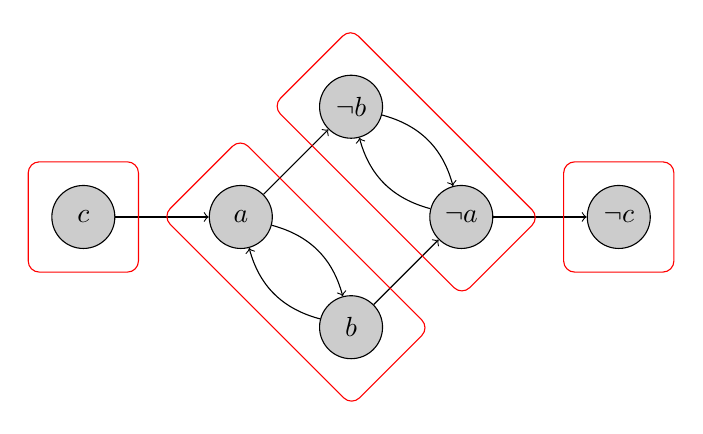
\begin{tikzpicture}[->,sibling distance=10em,
    every node/.style = {shape=circle, rounded corners,
        draw, align=center,minimum size=0.8cm,
    fill=black!20}]]
    \node (a) at (0, 0) {$a$};
    \node (b) at (1.4, -1.4) {$b$};
    \node (nb) at (1.4, 1.4) {$\lnot b$};
    \node (na) at (2.8, 0) {$\lnot a$};
    \node (c) at (-2, 0) {$c$};
    \node (nc) at (4.8, 0) {$\lnot c$};
    \path[every node/.style={font=\sffamily\small}]
        (a) edge[bend left] node[right] {} (b)
        (b) edge[bend left] node[right] {} (a)
        (c) edge node[right] {} (a)
        (a) edge node[right] {} (nb)
        (b) edge node[right] {} (na)
        (na) edge node[right] {} (nc)
        (na) edge[bend left] node[right] {} (nb)
        (nb) edge[bend left] node[right] {} (na);
    \draw[rounded corners, red] (-2.7, 0.7) rectangle (-1.3, -0.7);
    \draw[rounded corners, red] (4.1, 0.7) rectangle (5.5, -0.7);
    \draw[rounded corners, red, rotate around={-45:(0.7, -0.7)}] (-1, 0) rectangle (2.4, -1.4);
    \draw[rounded corners, red, rotate around={-45:(2.1, 0.7)}] (0.4, 0) rectangle (3.8, 1.4);
\end{tikzpicture}
\end{document}
